\documentclass[12pt]{article} %style de document
%utilisation du squelette latex de cours de l'an dernier
\usepackage[utf8]{inputenc} %encodage des caractères
\usepackage[french]{babel} %paquet de langue français
\usepackage[T1]{fontenc} %encodage de la police
\usepackage[top=2cm,bottom=2cm,left=2cm,right=2cm]{geometry} %marges
\usepackage{graphicx} %'affichage des images
\frenchbsetup{StandardLists=true}
\usepackage{enumitem}
\usepackage{amssymb}
\usepackage{fancyhdr}
\usepackage{graphicx}
\usepackage{dsfont}
\usepackage{upgreek}


\pagestyle{fancy}
\usepackage{xcolor} %ajouter couleur de fond
\definecolor{white}{RGB}{255,255,255}
\pagecolor{white}

\usepackage{cite}


\usepackage{verbatim}

\usepackage{hyperref}

%supprimer le trait du header
\renewcommand\headrulewidth{0pt}

%supprimer les endroits de footeur et header que l'on ne veut pas
\fancyfoot[L]{}
\fancyfoot[R]{}

\fancyhead[L]{}



\begin{document} %début du document
\begin{center}


\section*{Rapport projet M1 Hacking éthique}

Titouan LE BRET

Elouan MOELLO

M1 Cybersécurité

\bigskip


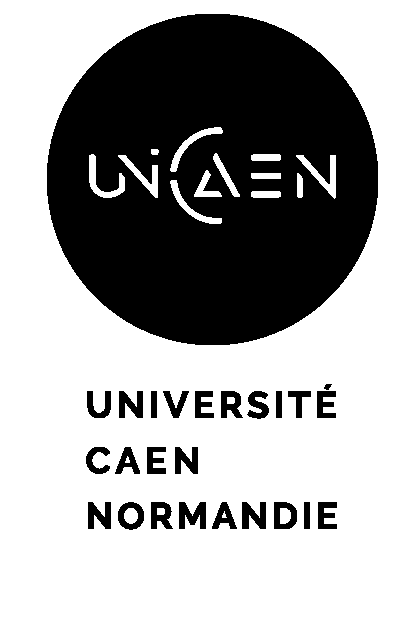
\includegraphics[scale=1.2]{images/LogoUNICAEN}
\begin{figure}[!h]
\label{}
\end{figure}
\end{center}



\newpage

\renewcommand{\contentsname}{Sommaire}
\tableofcontents




\newpage



\section{Introduction}
	\subsection{Présentation générale du projet}
		Contexte : réalisation d’un projet collaboratif dans le cadre du Master 1 Cybersécurité.
Explication des deux volets :
Site web Django pour la gestion d’inscriptions à une course.
Application Rust RSA pour explorer la sécurité et la validité des clés RSA.
Objectifs pédagogiques et techniques.
	
			
		
	\subsection{Organisation du projet}
		Rôles de chaque participant dans le développement des deux projets.
		Diagramme de gant (voir diapo)
	



\section{Conception générale}
	\subsection{Vision globale des deux projets}
		Description de chaque projet et de ses objectifs indépendants.
Justification de leur indépendance technique.

	
	\subsection{Cahier des charges}
		Site Django : gestion des inscriptions, sécurité des données et paiements.
Application Rust RSA : validation et tests de clés cryptographiques.

	
	\subsection{Contraintes et exigences}
		Sécurité, performance et adaptabilité des deux solutions.


\section{Développement du site Django}
	\subsection{Fonctionnalités principales}
		Inscriptions des utilisateurs.
Paiement sécurisé.
Intégration avec OAuth2 (Google).
Sécurisation des fichiers pdf.


	\subsection{Approche technique}
		Architecture Django : modèles, vues et templates.
Mise en œuvre de l’envoi d’e-mails.
Intégration du reCAPTCHA pour protéger les formulaires.
		
		
	\subsection{Sécurisation du site}
		Validation des données utilisateur.
Mesures pour protéger les fichiers 
Mesures de protection des paiements


	\subsection{Problèmes rencontrés et solutions}
		Difficultés techniques (exemple : configuration de SendGrid, gestion des fichiers).
Résolutions adoptées.
Problème communication en https et local


	\subsection{Axes d'améliorations}
		-Stockage des images en ligne (dans un DIsks sur render ou dans le CLoud google) -> demande abonnements payants
		-Implémentation paiement Stripe
		-
		

	

\section{Développement de l'application Rust RSA}
	\subsection{Objectifs et fonctionnalités principales}
		Tester la sécurité des clés RSA (validité, erreurs courantes).
Générer et valider des clés publiques.

	\subsection{Organisation technique}
		Structure des modules Rust (mod.rs, gestion des entrées).
Utilisation de rsa::BigUint pour les calculs.
Gestion des événements d’entrée/sortie et affichage des résultats.

	\subsection{Problèmes rencontrés et solutions}
		Gestion des entrées sans utiliser de String.

	\subsection{Axes d’amélioratrions }
		-Ajout de fonctions toujours possibiles sur les 2 pages
		-Ajout de 2 pages pour tester la signatures RSA 



\section{Conclusion et perspectives}
	\subsection{Différences fondamentales}
		Objectifs distincts : site orienté utilisateur, application centrée sur la cryptographie.
Langages et environnements de développement (Python/Django vs Rust).


	\subsection{Apport de chaque projet dans le cadre de la cybersécurité}
		Impact du site : mise en œuvre des bonnes pratiques de sécurité web + apprentissage django et d’API.
Impact de l’application : exploration de la cryptographie RSA et apprentissage de RUST
	
	
	
	\subsection{Bilan global}
		Synthèse des apprentissages.
Des améliorations possibles (projets évolutifs)



\section*{Annexes}
	\subsection{Codes sources importants}
		Extraits des parties clés de Django et Rust.
	\subsection{Ressources externes}
		Bibliographies, articles, et outils utilisés





\end{document}
